%++++++++++++++++++++++++++++++++++++++++
% Don't modify this section unless you know what you're doing!
\documentclass[letterpaper,12pt]{article}
\usepackage{tabularx} % extra features for tabular environment
\usepackage{amsmath}  % improve math presentation
\usepackage{graphicx} % takes care of graphic including machinery
\usepackage[margin=1in,letterpaper]{geometry} % decreases margins
\usepackage{cite} % takes care of citations
\usepackage[final]{hyperref} % adds hyper links inside the generated pdf file
\usepackage{pgfplotstable, booktabs}
\usepackage{placeins}
\usepackage{tabularray}
\usepackage{titlesec}
\usepackage{fancyhdr}
\usepackage{empheq}
\usepackage{amssymb}
\usepackage{sectsty}
\usepackage{tcolorbox}
\usepackage{listings}
\usepackage{xcolor}
\usepackage{parskip}
\usepackage{cancel}
\usepackage{enumitem}
\usepackage{amsmath}
\usepackage{mathrsfs}
\usepackage{physics}
\usepackage{subcaption}
\usepackage{pdfpages}
\usepackage{amsthm} 

\definecolor{codegreen}{rgb}{0,0.6,0}
\definecolor{codegray}{rgb}{0.5,0.5,0.5}
\definecolor{codepurple}{rgb}{0.58,0,0.82}

\lstdefinestyle{mystyle}{
    commentstyle=\color{codegreen},
    keywordstyle=\color{codepurple},
    numberstyle=\tiny\color{codegray},
    stringstyle=\color{codegreen},
    basicstyle=\ttfamily\small,
    breakatwhitespace=false,         
    breaklines=true,                 
    captionpos=b,                    
    keepspaces=true,                                                     
    showspaces=false,                
    showstringspaces=false,
    showtabs=false,                  
    tabsize=4
}

\lstset{style=mystyle}
  
\newcommand*\widefbox[1]{\fbox{\hspace{0em}#1\hspace{0em}}}
%define a divergence command which does \text{div}
\DeclareMathOperator{\Div}{Div}


\pagestyle{fancy}
\fancyhf{} % Clear all header and footer fields
\fancyhead[L]{MEC E 539}
%\fancyhead[C]{Center Header} 
\fancyhead[C]{Assignment 1}
\fancyhead[R]{Alex Diep}

\fancyfoot[C]{\thepage}

\pgfplotsset{compat=1.18} 
\titleformat*{\section}{\Large\bfseries}
\titleformat*{\subsection}{\large\bfseries}

\renewcommand{\thesection}{Question \arabic{section}}
\renewcommand{\thesubsection}{(\alph{subsection})}
\renewcommand*{\arraystretch}{1.5}

\hypersetup{
	colorlinks=true,       % false: boxed links; true: colored links
	linkcolor=blue,        % color of internal links
	citecolor=blue,        % color of links to bibliography
	filecolor=magenta,     % color of file links
	urlcolor=blue         
}
%++++++++++++++++++++++++++++++++++++++++
\begin{document}
% \begin{titlepage}
%     \centering
%     \vspace*{2cm} % Adjust vertical spacing
    
%     % Title
%     \Huge {MEC E 301 \\Lab 1: Dimensional Measurement} \\
%     \vspace{1cm} % Adjust vertical spacing
    
%     % Author
%     \Large by: Alex Diep \\
%     \vspace{1cm} % Adjust vertical spacing

%     % Date
%     \Large Date: September 19, 2023 \\ % or manually specify a date
%     \vspace{4cm} % Adjust vertical spacing

%     % CCID and Student ID in smtaller font
%     \normalsize CCID: abdiep \\
%     \normalsize Student ID: 1664334 \\ 
%     \normalsize Section: D21 \\
    
%     \vfill % Fill vertical space
    
%     % Additional content (e.g., university logo or other information)
    
% \end{titlepage}

\section{}
\textit{
The diagram models a gate valve which regulates the fluid flow in an engine. The gate valve is
modelled as a pendulum (with a massless rod and uniform disk of mass $m$ and radius $r$) pinned
to the engine at $R$, and is controlled by a spring/damper mechanism connecting the centre of the
disk to the engine.}

\textit{
    The engine's motion during operation is denoted as $y = A \sin (\omega t)$ , and the distance from $R$
    to the centre of the disk is $a$. Assuming small oscillations, the total horizontal displacement of
    the disk is denoted as $x$. The relative motion $z(t)$ between the gate and engine is given as:}
\[z = x - y = a\theta\]
\textit{Note: the disk is fixed to the rod, so it does not spin about the point of connection with the rod,
but the rod itself is pinned at $R$. For a uniform disk, $J = \frac{1}{2} m r^2$.}

\begin{figure}[H]
    \centering
    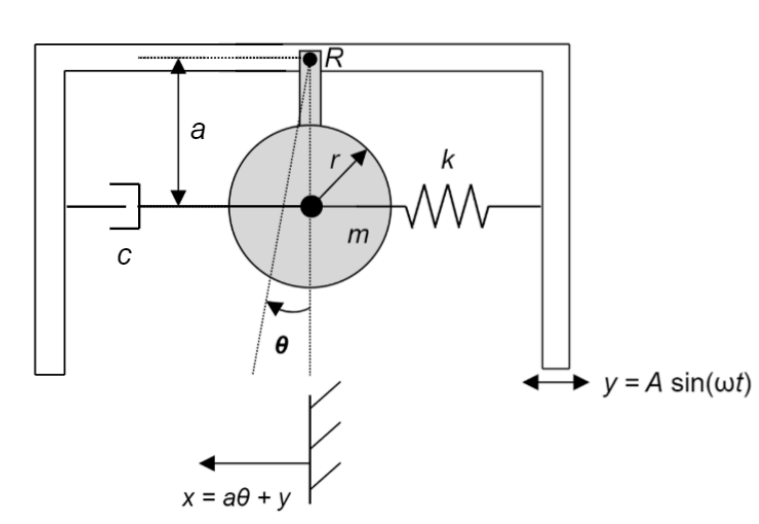
\includegraphics[width=0.5\linewidth]{Questions/Figures/Q1 Problem Diagram.png}
\end{figure}

\begin{enumerate}[label=(\alph*)]
    \item \textit{Determine the equation of motion for the relative motion of the gate with respect
    to the engine $z$, in terms of $m$, $k$, $a$, $g$, and $r$. Assume small oscillations.}
    \item \textit{If $\omega = 2400$ rpm, $a = 70$ mm, $r = 35$ mm, $m = 2.25$ kg, $k = 8.75$ kN/m, and
    $c = 30$ Ns/m, determine the amplitude of the relative motion $Z$ between the gate valve
    and engine in terms of $A$.}
\end{enumerate}

\subsection*{Solution}
\subsection{}
Here is the FBD and MAD for the problem:
\begin{figure}[H]
    \centering
    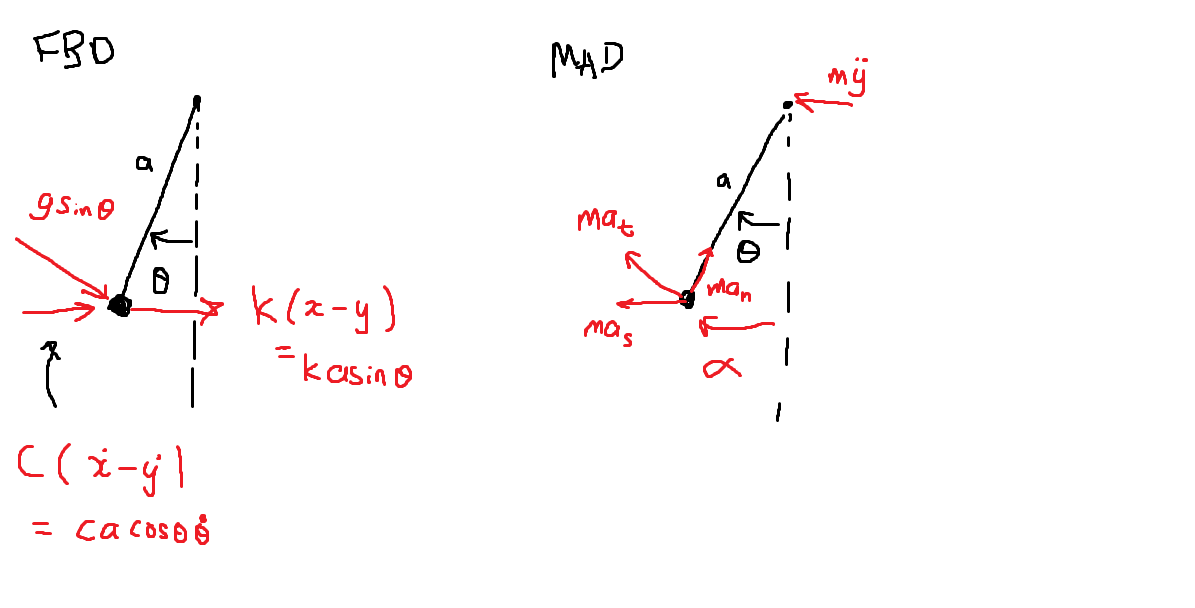
\includegraphics[width=0.8\linewidth]{Questions/Figures/Q1 FBD MAD.png}
\end{figure}

The equation of motion for the relative motion of the gate can be found by first taking the moment about the pin, $R$. Since the disk is undergoing rotation and translation, we consider general plane motion. First simplify the kinetic moment about the pin using the MAD diagram,
\begin{align}
    \circlearrowright \sum M_R &= (\mathcal{M}_k)_R \nonumber \\
    &= J_G \ddot{\theta}  + (a) m (a_G)_t  + (a \cos\theta) m (a_G)_s  \nonumber \\
    &= J_G \ddot{\theta} + ma (a\ddot{\theta})  + m(a \cos\theta) (\ddot{y})  \nonumber \\
    &= \underbrace{(J_G + m a^2)}_{J_{R}} \ddot{\theta} + m a \ddot{y} \cos\theta \label{eq:kinetic_moment}
\end{align}
Next, summing the moments in the FBD,
\begin{align}
    \circlearrowright \sum M_R &= -k a^2 \sin\theta - c a^2 \cos\theta \dot{\theta} - m g a \sin\theta \label{eq:force_moment}
\end{align}
Equating (\ref{eq:kinetic_moment}) and (\ref{eq:force_moment}), 
\begin{align*}
    J_R \ddot{\theta} + m a \ddot{y} \cos\theta &= -k a^2 \sin\theta - c a^2 \cos\theta \dot{\theta} - m g a \sin\theta
\end{align*}
Assuming small oscillations, we can use the small angle approximation, $\sin\theta \approx \theta$ and $\cos\theta \approx 1$ to simplify the equation.
\begin{align*}
    J_R \ddot{\theta} + m a \ddot{y} &= -k a^2 \theta - c a^2 \dot{\theta} - m g a \theta
\end{align*}
Rearranging,
\begin{align*}
    \left[J_R \right] \ddot{\theta} + \left[c a^2 \right] \dot{\theta} + \left[ k a^2 + m g a \right] \theta &= - m a \ddot{y}
\end{align*}
Since $z = a\theta$, multiplying both sides by $a$,
\begin{align*}
    \left[J_R \right] a \ddot{\theta} + \left[c a^2 \right] a \dot{\theta} + \left[ k a^2 + m g a \right] a \theta &= - m a^2 \ddot{y} \\
    \left[J_R \right] a z + \left[c a^2 \right] \dot{z} + \left[ k a^2 + m g a \right] z &= - m a^2 \ddot{y} 
\end{align*}
Finally,
\begin{align*}
    \Aboxed{\underbrace{\left[\frac{1}{2} m r^2 + m a^2 \right]}_{m_{\text{eff}}} \ddot{z} + \underbrace{\left[c a^2 \right]}_{c_{\text{eff}}} \dot{z} + \underbrace{\left[ k a^2 + m g a \right]}_{k_{\text{eff}}} z &= \underbrace{m a^2 A \omega^2}_{F_o} \sin(\omega t)}
\end{align*}

\subsection{}
This is the standard form of a forced, damped harmonic oscillator. From Eq. (5.9) in the textbook, the amplitude is 
\begin{align*}
    \mathbb{Z} &= \frac{F_o}{\sqrt{\left(k_{\text{eff}} - m_{\text{eff}} \omega^2 \right)^2 + \left(c_{\text{eff}} \omega \right)^2}}
\end{align*}
Determining the effective mass, damping, and stiffness,
\begin{align*}
    m_{\text{eff}} &= \frac{1}{2} m r^2 + m a^2 = \frac{1}{2} (2.25)(0.035)^2 + (2.25)(0.070)^2 = 0.0124 \\
    c_{\text{eff}} &= c a^2 = (30)(0.070)^2 = 0.147 \\
    k_{\text{eff}} &= k a^2 + m g a = (8.75\times 10^3)(0.070)^2 + (2.25)(9.81)(0.070) = 44.420\\
    F_o &= m a^2 A \omega^2 = (2.25)(0.070)^2 (2400 \times 2\pi / 60)^2 A= 696.3993 A
\end{align*}
Substituting into the amplitude equation,
\begin{align*}
    \mathbb{Z} &= \frac{696.3993}{\sqrt{\left(44.420 - 0.0124 (2400 \times 2\pi / 60)^2 \right)^2 + \left(0.147 (2400 \times 2\pi / 60) \right)^2}}A \\
    &= \boxed{0.9414 A}
\end{align*}
\section{}
\textit{Briefly describe the role of each component in determining the note that a string produces from a vibrational standpoint:}

\subsection{The fretboard}
The fretboard provides a surface for the guitarist to press down the strings against, effectively shortening the length of the vibrating portion of the string. By pressing the string against different frets, the guitarist changes the length of the vibrating portion, thereby altering the frequency of the produced note.

\subsection{The tuning pegs}
The tuning pegs are used to adjust the tension of the strings. Tightening or loosening the strings with the tuning pegs changes their tension, which in turn alters their fundamental frequency when plucked.

\subsection{The bridge}
The bridge of the guitar anchors the strings at the other end of the instrument. It also transmits the vibrations of the strings to the guitar body, contributing to the resonance and overall sound of the instrument.

\subsection{The frets}
The frets are unevenly spaced along the guitar neck to account for the logarithmic nature of musical intervals. The spacing between frets decreases as you move up the neck because the frequency ratio between notes is not linear. The spacing is designed according to the principles of equal temperament to ensure that each fret corresponds to the correct pitch on the musical scale.

\subsection{Bending a note}
Bending a note involves applying pressure to the string with one or more fingers and then moving the string across the fretboard horizontally, effectively increasing the tension and stretching the string. This action increases the pitch of the note being played. From a vibrational standpoint, bending a note alters the tension and length of the vibrating portion of the string, which in turn changes the fundamental frequency and pitch of the produced sound. Additionally, bending can introduce subtle variations in the harmonic content of the sound, adding expressiveness and character to the note.
% \section{}
National Institute of Nanotechnology (NINT) is a first generation Nano-research facility and the first of its kind in Canada. The facility is a six-storey building located on the University of Alberta Campus. Along with research offices, wet laboratories and clean nano-fab space, the facility features several ultra sensitive electron microscopes. In order for these microscopes to operate in the nanoscale, they must be provided with an extremely stable environment that is free from movement and vibration. One model of isolation setup for the electron microscopes is shown as (1) where an excitation displacement is applied to the base in response of floor vibration. The floor vibration is assumed to have a frequency of 50 Hz. The natural frequency of these whole setup is measured as 10 Hz.

\begin{figure}[h]
    \centering
    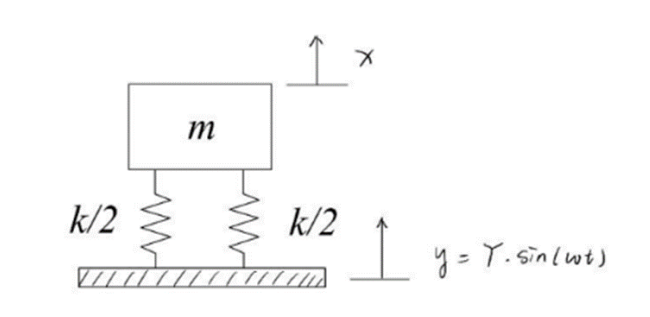
\includegraphics[width=0.5\textwidth]{Questions/Figures/q3 problem diagram.png}
\end{figure}

\begin{enumerate}[label=(\alph*)]
    \item (4 pts) Estimate the amplitude of vibration of electron microscope by comparing it to the amplitude of the floor for the setup as (1).
    \item (5 pts) The quality of the image from electron microscope is not satisfying since the amplitude is still too large. A dampler was added between the electron microscope and floor. What damping ratio should be chosen to make the amplitude of the vibration of electron microscope two times the amplitude in part a)?
    \item (1 pts) If the damping ratio of the damper needs to be adjusted to increase the amplitude of vibration of electron microscope, should the laboratory staff adjust the damping factor up or down?
\end{enumerate}

\subsection*{Solution}
\subsection{}
First, we decide the proper model for the problem. An appropriate model is an undamped SDOF system with base excitation. Since the springs are in parallel, the stiffness is $k_{\text{eff}} = k$. The DMF for this system is 
\begin{align*}
    \text{DMF} &= \frac{1}{1 - \left(\frac{\omega}{p}\right)^2}
\end{align*}
substituting,
\begin{align*}
    \text{DMF} &= \frac{1}{1 - \left(\frac{50}{10}\right)^2} \\
    &= \frac{1}{1 - 25} \\
    &= -0.04167
\end{align*}
This means that the amplitude of the electron microscope is $\boxed{4.167\%}$ of the amplitude of the floor. The negative sign indicated that the response of the electron microscope is 180 degrees out of phase with the floor.

\subsection{}
For a damped SDOF system with base excitation, the DMF is
\begin{align*}
    \text{DMF} &= \frac{\sqrt{1+\left(2\zeta\frac{\omega}{p}\right)^{2}}}{\sqrt{\left[1-\left(\frac{\omega}{p}\right)^{2}\right]^{2}+\left[2\zeta\frac{\omega}{p}\right]^{2}}}
\end{align*}
The DMF in a) was $1/24$, therefore we want the DMF to be $1/12$. 
\begin{align*}
    \frac{1}{12} &= \frac{\sqrt{1+\left(2\zeta\frac{50}{10}\right)^{2}}}{\sqrt{\left[1-\left(\frac{50}{10}\right)^{2}\right]^{2}+\left[2\zeta\frac{50}{10}\right]^{2}}} 
\end{align*}
Solving for $\zeta$,
\begin{verbatim}
syms zeta
eqn = 1/12 == sqrt(1+(2*zeta*5)^2)/sqrt((1-(5)^2)^2+(2*zeta*5)^2);
zeta = solve(eqn, zeta);
zeta = double(zeta)

>> zeta =
        -0.1738
         0.1738
\end{verbatim}
Therefore, the damping ratio should be $\boxed{0.1738}$.

\subsection{}
\begin{figure}[h]
    \centering
    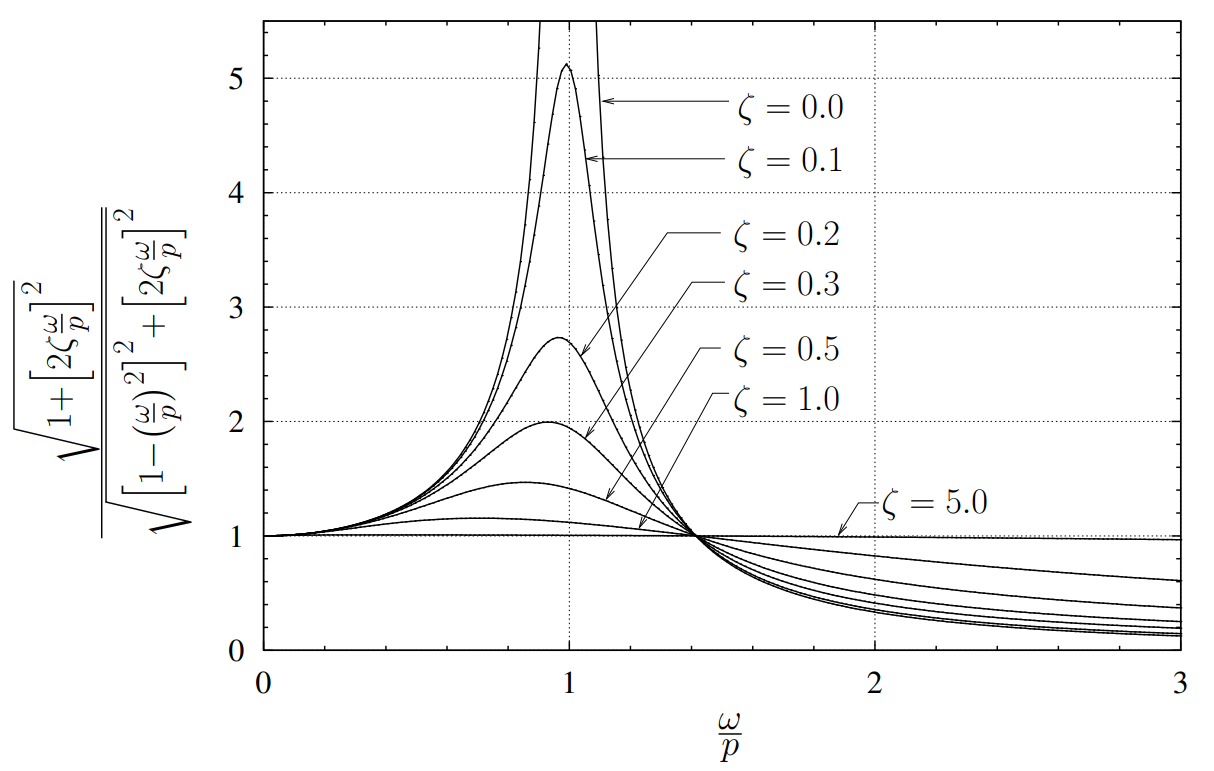
\includegraphics[width=0.5\textwidth]{Questions/Figures/q3 dmf diagram.png}
    \caption{Response amplitude of damped spring–mass system subjected to harmonic base
    excitation}
\end{figure}
Since we are operating on the RHS of the resonance peak, we should adjust the damping factor \textbf{up} to increase the amplitude of vibration of the electron microscope.
% \section{}
The figure shows a traction elevator system used in high-rise residential buildings. These traction 
elevators consist of hoist cables connected to the top of the cab operated by a traction machine 
(electric motor) located in the penthouse. The system is modelled as a simple spring-mass system, 
where the spring represents the cable stiffness and the mass corresponds to the elevator cab and its 
occupants (counterweights are neglected).
\begin{figure}[h]
    \centering
    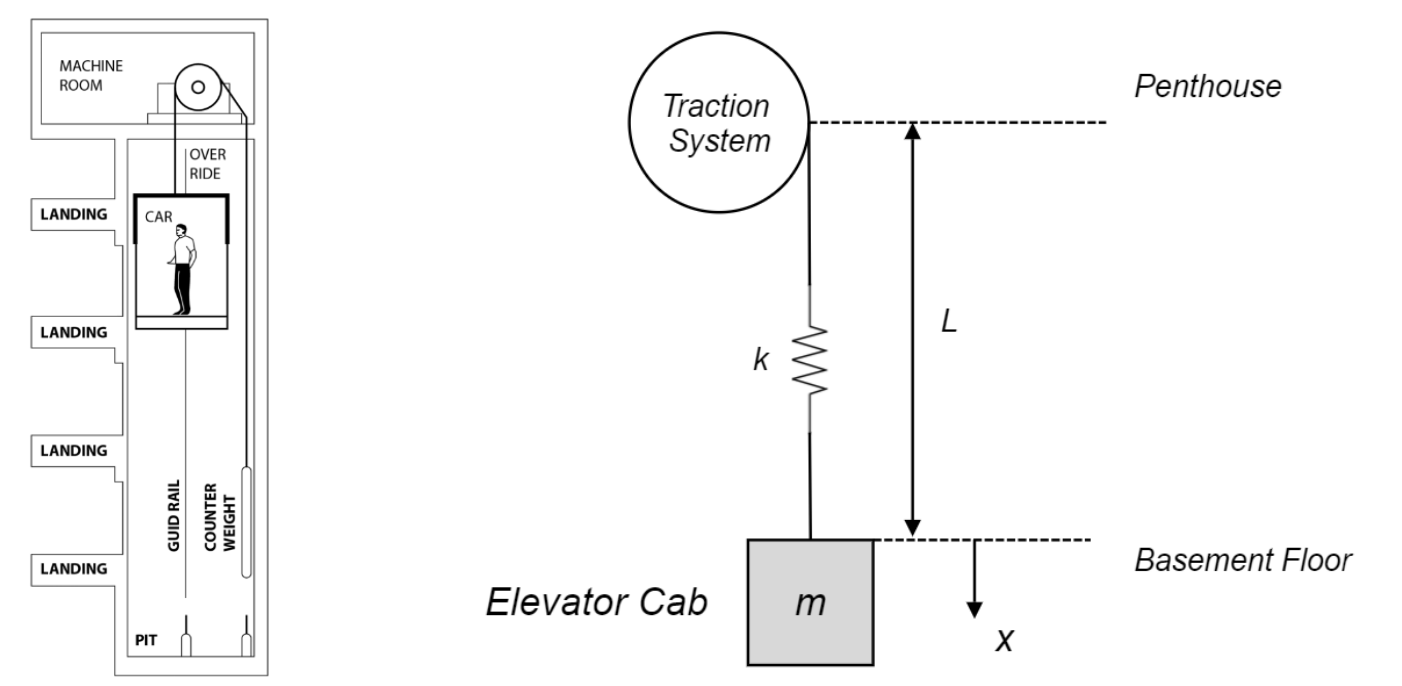
\includegraphics[width=0.5\linewidth]{Questions/Figures/q4 problem diagram.png}
    \caption{The traction elevator system}
    \label{fig:q4-png}
\end{figure}
The elevator provides a rapid ascent/descent, while not causing excessive acceleration to the
passengers or stress in the cable system. The situation under consideration is the stop after descent
to the basement floor level for a 10 floor apartment building (assume 3.5 m per story). Assume
that the traction motor stops instantly when reaching the basement floor (acts as a fixed support).
The velocity of the cab before stopping is 1.5 m/s. The cables have an equivalent stiffness of a
single cable with a radius of 2 cm and an elastic modulus of 100 GPa ($k = \frac{EA}{L}$).

\begin{enumerate}[label=(\alph*)]
    \item Consider both cases with an unloaded cab (mass of 1.2 metric tonnes) and with a maximum
        capacity of 15 people with an average weight of 70 kg each. For each case, determine:
        \begin{enumerate}[label=(\roman*)]
            \item (1 pt) The overshoot of the cab past the basement floor level after stopping.
            \item (1 pt) The maximum acceleration felt by the occupants.
            \item (1 pt) The maximum stress in the cables.
        \end{enumerate}
    \item (3 pts) To reduce the maximum tension in the cables and acceleration of the cab, a coil
        spring ($k = 600$ kN/m) is inserted between the cable attachment and the cab. How does
        this change the maximum displacement, acceleration, and stress for both the loaded and
        unloaded cases?
    \item The results for the vibration analysis of the original elevator system (no coil spring) was done
        under the assumption of no damping. However, the system components have an inherent
        damping. a test was done on an UNLOADED cab and it was found that the cab's oscillation
        amplitude decreased by 50\% in two cycles.
        \begin{enumerate}[label=(\roman*)]
            \item (2 pts) Determine the damping ratio for the LOADED case assuming viscous damping.
            \item (2 pts) For the LOADED case, estimate how much time is needed after reaching the ground
                floor so that the passengers feel virtually no vibration of the elevator cab. Assume that the
                vibrations essentially stop when the amplitude decreases to 8\% of its maximum value.
                Hint: recall that the logarithmic decrement is measured between subsequent peaks, so you
                must account for the time from $t = 0$ to the first peak.
        \end{enumerate}
\end{enumerate}

\subsection*{Solution}
\subsection{}
The system acts as a simple spring-mass system with initial conditions $x(0) = 0$ and $\dot{x}(0) = 1.5$ m/s. Assume that the equilibrium position is at the basement floor level.

The equation of motion is:
\begin{align*}
    \ddot{x} + \frac{k}{m} x &= 0
\end{align*}
with the general solution:
\begin{align*}
    x(t) &= A \cos (pt) + B \sin (pt)
\end{align*}
with the solution to the initial conditions:
\begin{align*}
    x(0) &= 0 \implies A = 0 \\
    \dot{x}(0) &= 1.5 \implies B = 1.5/p
\end{align*}
So the solution is:
\begin{align*}
    x(t) &= \frac{1.5}{p} \sin (pt)
\end{align*}
Next, the spring constant can be found by
\begin{align*}
    k &= \frac{EA}{L} = \frac{(100 \times 10^9) \pi (0.02)^2}{3.5 \times 10} = 3.59 \text{Mn/m}
\end{align*}
So the natural frequency for both cases is:
\begin{align*}
    p_{\text{unloaded}} &=  \sqrt{\frac{3.59 \times 10^6}{1200}} = 54.7 \text{rad/s} \\
    p_{\text{loaded}} &=  \sqrt{\frac{3.59 \times 10^6}{1200 + 15 \times 70}} = 39.9 \text{rad/s}
\end{align*}

The overshoot of the cab is simply the amplitude of the solution. So,
\begin{empheq}[box=\fbox]{align*}
    x_{\text{unloaded}, \text{overshoot}} &= \frac{1.5}{54.7} = 0.0274 \text{m} \\
    x_{\text{loaded}, \text{overshoot}} &= \frac{1.5}{39.9} = 0.0376 \text{m}
\end{empheq}

To find the maximum acceleration, we can take the second derivative of the solution 
\begin{align*}
    \ddot{x} &= -1.5 p \cos (pt)
\end{align*}
The maximum acceleration is the amplitude of the second derivative. So,
\begin{empheq}[box=\fbox]{align*}
    \ddot{x}_{\text{unloaded}, \text{max}} &= 1.5 \times 54.7 = 82.0 \text{m/s}^2 \\
    \ddot{x}_{\text{loaded}, \text{max}} &= 1.5 \times 39.9 = 59.9 \text{m/s}^2
\end{empheq}
The maximum stress in the cables is at the maximum displacement. So,
\begin{align*}
    \sigma_{\text{max}} &= \frac{k}{A} x_{\text{max}}  
\end{align*}
\begin{empheq}[box=\fbox]{align*}
    \implies \sigma_{\text{unloaded}, \text{max}} &= \frac{3.59 \times 10^6}{\pi (0.02)^2} \times 0.0274 = 78.35 \text{MPa} \\
    \implies \sigma_{\text{loaded}, \text{max}} &= \frac{3.59 \times 10^6}{\pi (0.02)^2} \times 0.0376 = 107.3 \text{MPa}
\end{empheq}

\subsection{}
An additional spring is added in series with the cable. For a simple oscillator, as seen in the Effective Stiffness Examples.pdf, the effective stiffness is given by:
\begin{align*}
    k_{\text{eff}} &= \frac{k_1 k_2}{k_1 + k_2}
\end{align*}
So the effective stiffness is:
\begin{align*}
    k_{\text{eff}} &= \frac{3.59 \times 10^6 \times 600 \times 10^3}{3.59 \times 10^6 + 600 \times 10^3} = 0.514 \text{Mn/m}
\end{align*}
So the new natural frequency for both cases is:
\begin{align*}
    p_{\text{unloaded}} &=  \sqrt{\frac{0.514 \times 10^6}{1200}} = 20.70 \text{rad/s} \\
    p_{\text{loaded}} &=  \sqrt{\frac{0.514 \times 10^6}{1200 + 15 \times 70}} = 15.1 \text{rad/s}
\end{align*}
The overshoot of the cab is 
\begin{empheq}[box=\fbox]{align*}
    x_{\text{unloaded}, \text{overshoot}} &= \frac{1.5}{20.70} = 0.0725 \text{m} \\
    x_{\text{loaded}, \text{overshoot}} &= \frac{1.5}{15.1} = 0.0993 \text{m}
\end{empheq}
The maximum acceleration is
\begin{empheq}[box=\fbox]{align*}
    \ddot{x}_{\text{unloaded}, \text{max}} &= 1.5 \times 20.70 = 31.1 \text{m/s}^2 \\
    \ddot{x}_{\text{loaded}, \text{max}} &= 1.5 \times 15.1 = 22.7 \text{m/s}^2
\end{empheq}
The maximum stress in the cables is at the maximum displacement. So,
\begin{align*}
    \sigma_{\text{max}} &= \frac{k}{A} x_{\text{max}}
\end{align*}
\begin{empheq}[box=\fbox]{align*}
    \implies \sigma_{\text{unloaded}, \text{max}} &= \frac{0.514 \times 10^6}{\pi (0.02)^2} \times 0.0725 = 29.7 \text{MPa} \\
    \implies \sigma_{\text{loaded}, \text{max}} &= \frac{0.514 \times 10^6}{\pi (0.02)^2} \times 0.0993 = 40.6 \text{MPa}
\end{empheq}

\subsection{}
Using the unloaded system, the damping ratio can be found through the logarithmic decrement (eq. 3.19).
\begin{align*}
    \delta &= \ln\left(\frac{x_1}{x_2}\right) \\
    \zeta &= \frac{\delta}{\sqrt{4\pi^2 + \delta^2}}
\end{align*}
where $x_1$ and $x_2$ are the amplitudes of the first and second peaks respectively. So then,
\begin{align*}
    \delta &= \ln\left(\frac{0.0274}{0.0274 \times 0.5}\right) = 0.6931 \\
    \zeta &= \frac{0.6931}{\sqrt{4\pi^2 + 0.6931^2}} = 0.1096 
\end{align*}
From the definition of the damping ratio, 
\begin{align*}
    \zeta &= \frac{c}{2mp}
\end{align*}
So the damping coefficient is:
\begin{align*}
    c &= 2mp\zeta = 2 \times 1200 \times 54.7 \times 0.1096 = 14388.3 \text{N s/m}
\end{align*}
Calculating the damping ratio for the loaded case,
\begin{empheq}[box=\fbox]{align*}
    \zeta &= \frac{c}{2mp} \\
    &= \frac{14388.3}{2 \times (1200 + 15 \times 70) \times 39.9} \\
    &= 0.0801
\end{empheq}

\subsection{}
For the time to reach 8\% of the maximum amplitude, (eq. 3.20) can be used to find the time from the zeroth peak to the m-th peak.
\begin{align*}
    \frac{\ln(x_n / x_{n+m}) \sqrt{1 - \zeta^2}}{2\pi\zeta} &= m 
\end{align*}
then let $x_n/x_{n+m} = 1/0.08 = 12.5$. So,
\begin{align*}
    m &= \frac{\ln(12.5) \sqrt{1 - 0.0801^2}}{2\pi \times 0.0801} = 5.00
\end{align*}
so the time can be found by
\begin{align*}
    \Aboxed{t &= m \tau = 5 \times \frac{2\pi}{\sqrt{1- \zeta^2}p} = 5 \times \frac{2\pi}{\sqrt{1- 0.0801^2} \times 39.9} = 0.790 \text{s}}
\end{align*}

% \section{}

% Two degree of freedom system shown consists of a rigid bar AC of negligible mass, disc of mass 
% 𝑚1 which is pinned at C and rolls without slipping on the wall, and a mass 𝑚2 suspended by a 
% spring of stiffness 𝑘2. 
\textit{The two degree of freedom system shown consists of a rigid bar AC of negligible mass, disc of mass $m_1$ which is pinned at C and rolls without slipping on the wall, and a mass $m_2$ suspended by a spring of stiffness $k_2$.}
\begin{figure}[H]
    \centering
    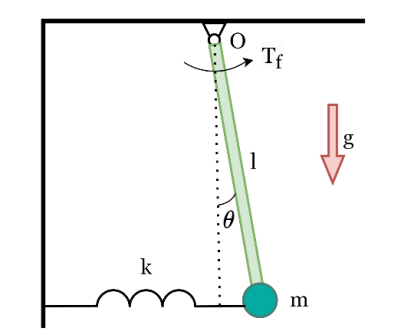
\includegraphics[width=0.5\textwidth]{Questions/Figures/Q5 Problem Diagram.png}
    \caption{Two degree of freedom system}
\end{figure}

% \textit{For the general case of 𝑚1, 𝑚2, 𝑘1, 𝑘2 determine the equations of motion. Be sure 
% to include a detailed free-body diagram. }
\textit{For the general case of $m_1$, $m_2$, $k_1$, $k_2$ determine the equations of motion. Be sure to include a detailed free-body diagram.}
\begin{figure}[H]
    \centering
    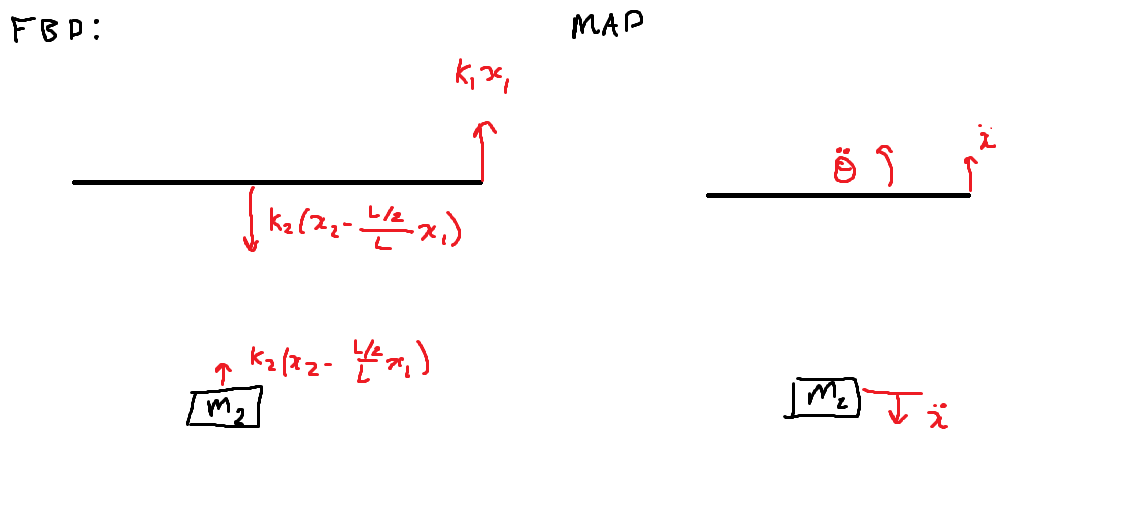
\includegraphics[width=0.5\textwidth]{Questions/Figures/Q5 FBD.png}
    \caption{Free-body diagram}
\end{figure}

Summing the moment about the pivot point, $A$, 
\begin{align*}
    \circlearrowright \sum M_A :&= J_A \alpha = (m_1 r^2 + m_1 L^2) \ddot{\theta} \\
    &= + k_2 \left(x_2 - \frac{1}{2} x_1 \right) \left(\frac{L}{2}\right) - k_1 x_1 L \\
    &= k_2 x_2 \frac{L}{2} - k_2 \frac{L}{4} x_1 - k_1 x_1 L
\end{align*}
using $\theta = x_1/r$, 
\begin{align*}
    (m_1 r^2 + m_1 L^2) \frac{\ddot{x}_1}{r} + k_1 x_1 L + k_2 \frac{L}{4} x_1 - k_2 x_2 \frac{L}{2} &= 0 \\
    \left[\frac{1}{r} \left(m_1 r^2 + m_1 L^2\right)\right] \ddot{x}_1 + \left[k_1 L + k_2 \frac{L}{4}\right] x_1 - k_2 x_2 \frac{L}{2} &= 0
\end{align*}
Summing the forces in the $y$ direction of the mass, $m_2$,
\begin{align*}
    \downarrow \sum F_y :&= m_2 \ddot{x}_2 \\
    &= - k_2 (x_2 - \frac{L}{2}x_1)
\end{align*}
then,
\begin{align*}
    m_2 \ddot{x}_2 + k_2 x_2 - k_2 \frac{L}{2} x_1 &= 0
\end{align*}
The equations of motion are then,
\begin{align*}
    \begin{bmatrix}
        \left[\frac{1}{r} \left(m_1 r^2 + m_1 L^2\right)\right] & 0 \\
        0 & m_2
    \end{bmatrix}
    \begin{Bmatrix}
        \ddot{x}_1 \\
        \ddot{x}_2
    \end{Bmatrix}
    +
    \begin{bmatrix}
        k_1 L + k_2 \frac{L}{4} & -k_2 \frac{L}{2} \\
        \frac{-k_2 L}{2} & k_2
    \end{bmatrix}
    \begin{Bmatrix}
        x_1 \\
        x_2
    \end{Bmatrix}
    &=
    \begin{Bmatrix}
        0 \\
        0
    \end{Bmatrix}
\end{align*}

% (5 pts) If 𝑘1 = 𝑘2 = 𝑘 and 𝑚1 = 𝑚2 = 𝑚, determine the natural frequencies and 
% corresponding mode shape
\subsection{}
\textit{If $k_1 = k_2 = k$ and $m_1 = m_2 = m$, determine the natural frequencies and corresponding mode shape.}
By Matlab,
\begin{verbatim}
syms k m L r
M = [1/r*(m*r^2 + m*L^2), 0; 0, m];
K = [k*L + k*L/4, -k*L/2; -k*L/2, k];
[V, D] = eig(inv(M)*K);
p = simplify(D)
simplify(V)
\end{verbatim}

The natural frequencies are,
\begin{empheq}[box=\fbox]{align*}
    p_1 &= 0.412 \frac{k}{m} \\
    p_2 &= 1.213 \frac{k}{m}
\end{empheq}
And the corresponding mode shapes are,
\begin{empheq}[box=\fbox]{align*}
    \Phi^{\textcircled{1}} &= \begin{Bmatrix} 0.851 \\ 1 \end{Bmatrix} \\
    \Phi^{\textcircled{2}} &= \begin{Bmatrix} -2.351 \\ 1 \end{Bmatrix}
\end{empheq}

% \newpage
% %\bibliographystyle{IEEEtran}
% %\bibliography{citations.bib}
% %\bibliography{}

% \newpage
% \appendix
% \sectionfont{\large}
\section{Appendix: Matplotlib Python Code to Render Graphs}
This is just some random code.
\begin{lstlisting}[language=Python]
if transactions: Transaction.create_transactions() # if transactions = "true"
node.generate_emptyState() # empty state for all nodes
S.initial_events() # initiate initial events to start with

while not queue.isEmpty() and clock <= targetTime:
    next_e = queue.get_next_event()
    clock = next_e.time # move clock to the time of the event
    Event.execute_event(next_e)
    Queue.remove_event(next_e)

print results
\end{lstlisting}

\end{document}